%----------------------------------------------------------------------------------------
%	PACKAGES AND OTHER DOCUMENT CONFIGURATIONS
%	DONT CHANGE !
%----------------------------------------------------------------------------------------
\documentclass{report}
\newcommand*{\plogo}{\fbox{$\mathcal{PL}$}} % Generic publisher logo
\usepackage[portuguese]{babel}
\usepackage[utf8]{inputenc}
\usepackage{verbatim}
\usepackage{amsmath}
\usepackage{amsfonts}
\usepackage{listings}
\usepackage{hyperref}
\usepackage{xcolor}
\usepackage{color}
\usepackage{varwidth}
\usepackage{graphicx}
\usepackage{mathtools}

%----------------------------------------------------------------------------------------
%	TITLE PAGE
%----------------------------------------------------------------------------------------

\newcommand*{\titleGP}{\begingroup % Create the command for including the title page in the document
\centering						 % Center all text
\vspace*{\baselineskip} 			 % White space at the top of the page

\rule{\textwidth}{1.6pt}\vspace*{-\baselineskip}\vspace*{2pt} 	% Thick horizontal line
\rule{\textwidth}{0.4pt}\\[\baselineskip] 					% Thin horizontal line

{\LARGE THE BIG BOOK\\ OF \\[0.3\baselineskip] ROBOTA}\\[0.2\baselineskip] % Title

\rule{\textwidth}{0.4pt}\vspace*{-\baselineskip}\vspace{3.2pt} % Thin horizontal line
\rule{\textwidth}{1.6pt}\\[\baselineskip] 					% Thick horizontal line

\scshape % Small caps
A number of fascinating and life-changing works \\ 		% Tagline(s) or further description
presented  in a clear and useable way \\[\baselineskip] 	% Tagline(s) or further description
Florian\'opolis,  2013--inf \par 							% Location and year
\vspace*{2\baselineskip} 									% Whitespace between location/year and editors

Edited by \\[\baselineskip]
{\Large Felippe Schmoeller \\ Martin Vincent \\ Patrick J.P \\ \par} 		% Editor list
{\itshape The University of \\ Santa Catarina\par} 	% Editor affiliation

\vfill % Whitespace between editor names and publisher logo

\plogo \\[0.3\baselineskip] 			% Publisher logo
{\scshape 2013} \\[0.3\baselineskip]  % Year published
{\large ROBOTA}\par \endgroup}            % Publisher


\newcommand{\blankpage}{
\newpage
\thispagestyle{empty}
\mbox{}
\newpage
}
%----------------------------------------------------------------------------------------
%	DOCUMENT
%----------------------------------------------------------------------------------------

\begin{document} 

\titleGP % This command includes the title page

\newpage

\tableofcontents  % This command put the sections and subsections

%----------------------------------------------------------------------------------------
%   LE MASTER INCLUDE
%----------------------------------------------------------------------------------------

%----------------------------------------------------------------------------------------
%	THE BIG BOOK OF ROBOT BEGIN HERE
%----------------------------------------------------------------------------------------


%----------------------------------------------------------------------------------------
% INTRODUCTION
\newpage
\chapter{Introdução}

% declara a section
\section{Introduç\~ao ao livro.} % declarando uma section.
Esse livro tem como objetivo armazenar todo o conhecimento do grupo ROBOTA,
ajudando novos membros e colaborando com o ambiente acadêmico.

%declara a subsection
\subsection{Sobre THE BIG BOOK OF ROBOTA.}	% declarando uma subsection.
Esse livro teve inicio no fatídico dia (04/11/2013) para maior organizaç\~ao do grupo,
unir toda a documentaç\~ao e evitar o retrabalho.

Este livro esta separado em 5 capítulos:

% enumerando alguns tópicos
\begin{enumerate}
\item Introdução
\item Software
\item Hardware
\item Mecânica
\item Gerencial
\end{enumerate}

Cada capitulo possui uma pasta e cada pasta possui outra para as seções, como mostrado na fugira \ref{estrutura}.

% adicionando uma figura
% o caminho da figura tem que ser des da raiz.

\begin{center}
\center
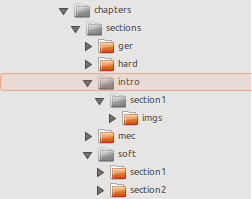
\includegraphics[width=6cm]{./include/chapters/sections/intro/section1/imgs/estrutura.png}

\section{Estrura de pastas.}
\label{estrutura}
\end{center}

Essa estrutura pode ser detalhada da seguinte forma:\\										% serve para quebrar a linha
A pasta raiz do THE BIG BOOK OF ROBOTA contem a pasta include, que por sue vez contem a pasta chapters,
cada aquivo tex dentro desta pasta possui os caminhos para sections.\\

Assim, caso algu\'em queira adicionar mais um arquivo ao grandioso e inigualável THE BIG BOOK OF ROBOTA, 
\'e s\'o seguir o que \'e dito na proxima subsection (~\ref{subsec:adicionandosuacontribuicao}).		% referenciando o label

\subsection{Adicionando sua contribuição.} ~\label{subsec:adicionandosuacontribuicao}			% adicionando um label para ser referenciado

Bem, vamos l\'a, primeiramente podes utilizar essa pr\'opria section como exemplo, ela est\'a em:\\
root/include/chapters/sections/intro/section1\\													
Podendo encontrar o arquivo tex, esse seria como um ambiente de trabalho, onde existe o seu tex
e uma pasta para imagens da sua section. \\
Após criar seu tex, vamos adicionar ele ao nosso livro.\\
Primeiramente vá até: 
root/include/chapters/\\
Entre no tex do capitulo que gostaria adicionar seu tex, agora é só adicionar a seguinte linha ao documento:\\
input\{./include/chapters/sections/XXX/sectionX/section.tex\}\\
Onde XXX seria o nome da pasta do capitulo e X o numero da section.\\
Simplificando seria os seguintes paços:\\

% enumerando paços
\begin{enumerate}
\item Crie seu .tex 
\item Dentro da pasta sections, entre na pasta do chapter que gostaria de adicionar e crie uma pasta sectionX para adicionar seu .tex 
\item Ap\'os adicionar seu arquivo, inclua o caminho dele dentro da arquivo .tex como exemplificado dentro de intro.tex
\item N\~ao esqueça de quando for compilar, sempre compilar o arquivo main.tex, não o arquivo .tex da section !!
\end{enumerate}

\author{Patrick J.P}		% adicionando um autor




%----------------------------------------------------------------------------------------
% SOFTWARE
\newpage
\chapter{Software}

Parte de Software, com algumas informações sobre controle de versão, servidores remotos de versão, Arduino e documentação Doxygen.

\section{Controle de vers\~ao}
\subsection{Git}
O GIT é um sistema de controle de versão, de código aberto, tendo como um dos desenvolvedores o conhecido Linus Torvalds.
\begin{quote}
Eu sou um egoísta degenerado, batizo todos os meus projetos com meu nome. Primeiro Linux, agora Git.
— Linus Torvalds
\end{quote}
Lembrando que Git é um gíria para cabeça dura, contudo podendo ter outros sinônimos como: Global information tracker, ou, quando ele trava, ``Goddamn idiotic truckload of sh*t".

\begin{center}
\center
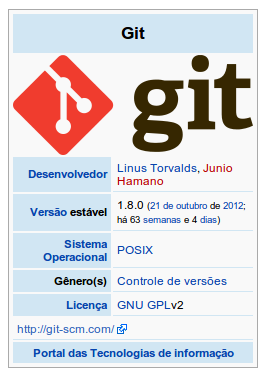
\includegraphics[width=6cm]{./include/chapters/sections/soft/section1/img/git.png}
\label{git wiki}
\end{center}

Uma ferramente de controle de versão possui uma série de periféricos para possibilitar sua utilização, nesta parte iremos introduzir algumas delas.

\begin{enumerate}
\item Criando \\
Para criar um repositório local: git init\\
Para clonar um repositório remoto: git clone  /caminho/para/o/repositório\\
Para clonar um repositório remoto: git clone username@host:/caminho/para/o/repositório ou git clone\\ https://github.com/username/repositório.git\\

\item Adicionando e removendo \\
Para adicionar arquivos no repositório a ser verificado: git add nome\_do\_arquivo
Para adicionar tudo ao repositório: git add *
Para remover um arquivo do repositório: git rm nome\_do\_arquivo

\item Commit (comentar as mudanças) e sincronizar \\
Commitar mudanças: git commit -m ``mensagem de commit"\\
Atualizar o seu repositório: git pull\\
Atualizar o repositório remoto: git push\\
Conectar repositório local com um remoto: git remote add origin server\\

\item Branches (ramos no repositório) \\
Criar um novo branche: git checkout -b nome\_do\_branch\\
Trocar do branch para o master: git checkout master\\
Deletar branch: git branch -d nome\_do\_branch\\
Dar um push do branch para o repositório local: git push origin branch\\

\item Merges (incorporar mudanças) \\
Merge as mudanças de algum branch: git merge nome\_do\_branch\\
Vê as mudanças entre dois branches: git diff branch\_fonte branch\_alvo\\

\end{enumerate}

\begin{figure}[!htb]
\centering
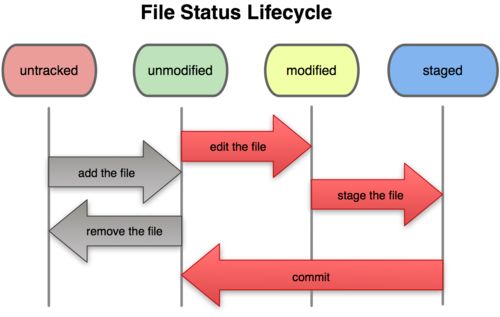
\includegraphics[width=11cm]{./include/chapters/sections/soft/section1/img/filestatus.png}
\caption{Ciclo GIT}
\label{CicloVidaGit}
\end{figure}

A figura \ref{CicloVidaGit}, mostra numa vis\~ao muito simplificada a utiliza\c{c}\~ao do git. \\
Tendo como in\'icio, o arquivo n\~ao rastreado, ``untracked", temos que iniciar o mesmo no reposit\'orio, para isso utilizando o comando: \\ \$ git add nome\_do\_arquivo, \$ git add * ou at\'e mesmo \$ git add $--$all. \\ \\
Tendo em m\~aos o arquivo modificado, organize e comente o mesmo para o commit, fazendo assim uma atualiza\c{c}\~ao do arquivo para o gerenciador de vers\~ao, desta forma o arquivo ira constar como atualizado na sua maquina para ultima vers\~ao, desta forma, basta utilizar o seguinte comando:\\ \$ git commit -m ``mensagem", \$ git commit e escrever a mensagem em seguida.\\ \\
Fazendo tudo isso na sua maquina e tendo o arquivo como n\~ao modificado, ``unmodified", est\'a na de atualizar o servidor remoto, utilizando desta forma o comando: \\
\$ git push origin master \\ \\


\subsection{Primeiros passos}
\begin{enumerate}
\item Configurando.\\
Após a instalação do git.\\
Vamos fazer algumas configurações do usuario. \\
username:   \\
\$ git config --global user.name ``seu nome"  \\
Email:      \\
\$ git config --global user.name ``seu\_mail@exemplo.com" \\

Esses dados são uteis, pois iram junto com seus commits.\\
Caso esteja utilizando o GitHub, é altamente aconselhável utilizar o mesmo e-mail para ambos.\\
Pode visualizar as modificações utilizando:\\
\$ git config --list

\item Conseguindo um repositório git.\\

a) Inicializando um repositório de um diretório existente.\\
\$ git init \\
Este comando cria um subdiretório .git, que ira conter todos os arquivos necessários para o git.\\
Após isso é necessário adicionar os arquivos que você gostaria de serem adicionados ao nosso repositório.\\
\$ git add README		\\
Após adicionar nossos arquivos, vamos agora comentar as modificações.\\
\$ git commit -m ``primeiro commit, adicionado os arquivos"\\
Terminando isso seu repositório Git esta pronto e atualizado, podendo ser visualizado pelo comando:\\
\$ gitk\\

b) Iniciando um repositório utilizando um existente.\\
Em sua essência utilizamos o comando:\\
\$ git clone url \\
Que, por sua vez, clona um repositório ja existente.\\
Ex: \$ git clone git://github.com/live/4ever.git\\
Como o ``\$ git init" ele também cria uma pasta .git que possui todo o  histórico e modificações do repositório.

\item Salvando modificações.\\
Para checar o status dos arquivos, utilizamos o comando:\\
\$ git status \\
Se o retorno for: nothing to commit (working directory clean),significa que seu repositório esta atualizado.\\
Caso for diferente, devemos atualizar o repositório e comentar as mudanças.\\
Para rastrear arquivos dentro do diretório, utilizamos o comando:\\
\$ git add \\
Caso todos os arquivos dentro da pasta estejam no diretório, é recomendado utilizar:\\
\$ git add --all\\
Arquivos específicos:\\
\$ git add README\\
Arquivos com extensão especifica:\\
\$ git add *.c\\

Para poder ver a situação atual do repositório utilizando o comando status do Git, ``\$ git status", 
permitindo desta forma visualizar modificaç\~oes depois do ultimo commit.
Utilizando o comando de status, poderemos ver:\\

Algumas extensões são ignoradas pelo comando ``\$ git add", geralmente são arquivos de compilação e temporários:\\
*.o\\
*.a\\
*$\sim$\\

Visualizando modificações.\\
A principal ferramenta para visualizar as modificações do ultimo commit é o comando ``\$ git diff", mostra os arquivos e linhas modificadas. A visualização é bem instintiva e de grande ajuda para os commits realizados no futuro.\\

Commitando as modificações.\\
Após adicionar o arquivo e modificar, vamos agora commitar as modificações, esta ação atualiza todos os arquivos rastreados pelo git,fazendo dessa forma um update do repositório local comentado.\\
O comando base:\\
\$ git commit\\
(Este comando utiliza da variável Shell \$EDITOR, vim,emacs,nano. Caso não esteja configurado no seu OS, utilize o comando ``\$ git config --global core.editor").

Abrindo tela, é possível deixar uma mensagem para comentar as atualizações.\\
Para tornar este comando mais pratico, existe a possibilidade de adicionar a variável -m.\\
Ex: \$ git commit -m ``o arquivo README foi modificado"\\

\item Visualizando o histórico do commit.\\

Após dar um clone num repositório, podemos visualizar todas os commits realizados durante sua existência utilizando o comando ``\$ git log".\\
Esta função do git, possui inúmeras funcionalidades e variáveis para ajudar o desenvolvedor, contudo existi uma ferramenta mais amigável:\\
\$ gitk\\
\begin{figure}[!htb]
\centering
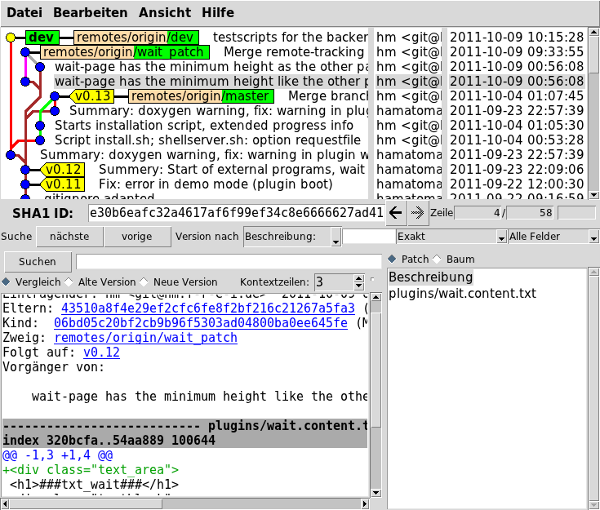
\includegraphics[width=11cm]{./include/chapters/sections/soft/section1/img/gitk.png}
\caption{Gitk}
\label{Gitk}
\end{figure}

\item Trabalhando com um repositório remoto.

Trabalhando num repositório remoto, abre as portas para novas oportunidades e colaboração entre os desenvolvedores.\\
Primeiramente, vamos clonar um repositório:\\
\$ git clone url\\
Este comando permite fazer uma c\'opia do reposit\'orio remoto para seu computador.\\
Você também pode adicionar a variável -v,podendo mostrar a url que foi retirada o repositório.\\
\$ git remote -v

Atualizando o repositório remoto.\\
Caso seu repositório local esta pronto, podemos enviar as modificações para o servidor remoto, utilizando o comando:\\
\$ git push origin master\\
(Tendo previamente definido.)\\

\item Marcações.\\

Utilizado geralmente para marcar a versão que estamos trabalhando no projeto (v1.0 e assim por diante), vamos agora dar alguns exemplos.\\
A listagem das tags pode ser feita utilizando o comando:\\
\$ git tag\\
\# v0.1 \\
\# v1.3\\
Este comando lista as marcas em ordem alfabética, a ordem em  que eles aparecem não possui nenhuma importância.

Criando Marcações.\\
Pode ser feito marcações (-a) com comentários (-m):\\
\$ git tag -a v1.4 -m 'minha versão 1.4'\\
\$ git tag\\
\# v0.1\\
\# v1.3\\
\# v1.4\\

Você pode visualizar as informações da marcação, com o comando:\\
\$ git tag show v1.4\\
\# tag v1.4\\
\# Tagger: Scott Chacon schacon@gee-mail.com\\
\# Date:   Mon Feb 9 14:45:11 2009 -0800\\
\# \\
\# my version 1.4\\
\# commit 15027957951b64cf874c3557a0f3547bd83b3ff6\\
\# Merge: 4a447f7... a6b4c97...\\
\# Author: Scott Chacon schacon@gee-mail.com\\
\# Date:   Sun Feb 8 19:02:46 2009 -0800\\
\# \\
\#     Merge branch 'experiment'\\
\# \\

Pode ser feita uma pesquisa rápida e limitada.\\
\$ git tag-l 'v1.4.2. *' \\
\# v1.4.2.1 \\
\# v1.4.2.2 \\
\# v1.4.2.3 \\
\# v1.4.2.4\\

Compartilhando marcações.\\
Por padrão o comando ``\$ git push" não transfere tags para servidores remotos.\\
A maneira existente para fazer isso, seria utilizar o comando no formato:\\
\$ git push origin nome\_da\_tag\\
Ex: \$ git push origin v1.5\\
\# Counting objects: 50, done.\\
\# Compressing objects: 100\% (38/38), done.\\
\# Writing objects: 100\% (44/44), 4.56 KiB, done.\\
\# Total 44 (delta 18), reused 8 (delta 1)\\
\# To git@github.com:schacon/simplegit.git\\
\# * [new tag]         v1.5 - v1.5\\

Se existe um numero grande de marcações que gostaria de dar push, pode utilizar --tags como opção.\\
\$ git push origin --tags\\
\# Counting objects: 50, done.\\
\# Compressing objects: 100\% (38/38), done.\\
\# Writing objects: 100\% (44/44), 4.56 KiB, done.\\
\# Total 44 (delta 18), reused 8 (delta 1)\\
\# To git@github.com:schacon/simplegit.git\\
\#  * [new tag]         v0.1 - v0.1\\
\#  * [new tag]         v1.2 - v1.2\\
\#  * [new tag]         v1.4 - v1.4\\
\#  * [new tag]         v1.5 - v1.5\\
\end{enumerate}

\subsection{Ramificações ou Branchs}

O Branch pode ser simplesmente definido como:
\begin{quote}
Um branch no Git é simplesmente um leve ponteiro móvel para um desses commits. O nome do branch padrão no Git é master. Como você inicialmente fez commits, você tem um branch principal (master branch) que aponta para o último commit que você fez. Cada vez que você faz um commit ele avança automaticamente. 
— \href{http://git-scm.com/book/pt-br/Ramifica\%C3\%A7\%C3\%A3o-Branching-no-Git-O-que-\%C3\%A9-um-Branch}{git-scm}
\end{quote}

A figura \ref{Branch} exemplifica como funciona na pratica, o branch da inicio no ultimo commit e quando terminado o objetivo dele, as modificações são aplicadas ao master.

\begin{figure}[!htb]
\centering
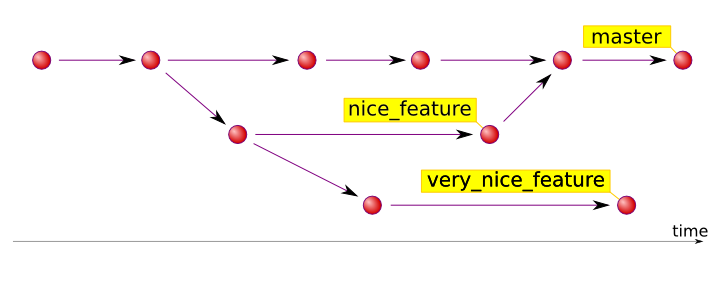
\includegraphics[width=11cm]{./include/chapters/sections/soft/section1/img/branch.png}
\caption{Exemplo de Branch}
\label{Branch}
\end{figure}

Para criar um Branch basta utilizar o comando:\\
\$ git checkout -b  nome\_do\_branch\\
\$ git branch  nome\_do\_branch\\
Ex: \$ git checkout -b nice\_feature\\
Ex: \$ git branch nice\_feature\\

Para nosso diret\'orio apontar para o novo branch, devemos utilizar o comando:\\
\$ git checkout nome\_do\_branch\\
Ex:\$ git checkout nice\_feature\\

Como pode ser visto na figura \ref{checkout}, podemos ver que com o checkout mudamos o local do ponteiro onde estamos trabalhando, desta forma, as modificaç\~oes serão feitas aonde o apontador esta localizado.

\begin{figure}[!htb]
\centering
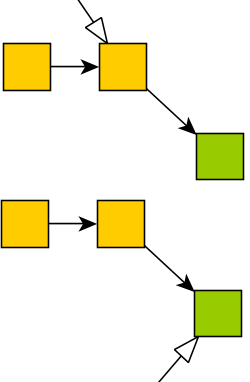
\includegraphics[width=4cm]{./include/chapters/sections/soft/section1/img/apontador3.png}
\caption{Exemplo checkout}
\label{checkout}
\end{figure}
Ap\'os as modificaç\~oes serem realizadas, esta na hora de integrar as modificaç\~oes com o branch master.\\

Primeiramente, devemos estar com o nosso apontador no master:\\
\$ git checkout master\\
Em seguida, fazer o merge e atualizar nosso master com a nice\_feature:\\
\$ git merge - -no-ff nice\_feature\\
\# Merge made by recursive.\\
\# README | 1 +\\
\# 1 files changed, 1 insertions(+), 0 deletions(-)\\

É recomendado que utilize o comando ``\$ git merge - -no-ff nice\_feature" com a opção - -no-ff, pois:
\begin{quote}
Isso evita a perda de informações sobre a existência histórica de um ramo e suas características, junto com todos os commits.
— \href{http://nvie.com/posts/a-successful-git-branching-model/}{nvie}
\end{quote}

A figura \ref{noff} exemplifica bem a diferença.\\
\begin{figure}[!htb]
\centering
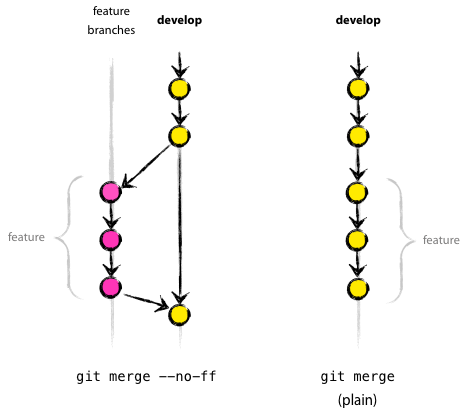
\includegraphics[width=9cm]{./include/chapters/sections/soft/section1/img/off.png}
\caption{Exemplo da opç\~ao - -no-ff}
\label{noff}
\end{figure}

Com a atualização do seu master, não existe mais a necessidade de ter ainda em paralelo o branch,
assim podemos deletar o mesmo, utilizando o comando:\\
\$ git branch -d nome\_do\_branch\\
Ex: \$ git branch -d nice\_feature\\

Conflitos de Merge.

Como visto na figura \ref{checkout}, temos em paralelo o branch nice\_feature com o branch very\_nice\_feature.
Contudo, pode acontecer alguns problemas, se for alterada a mesma parte do mesmo arquivo de forma diferente nos dois branches, o Git não será capaz de executar o merge  de forma clara, o conflito pode ser demostrado com:\\
\$ git merge very\_nice\_feature\\
\# Auto-merging index.html\\
\# CONFLICT (content): Merge conflict in index.html\\
\# Automatic merge failed; fix conflicts and then commit the result.\\

Todo conflito de merge que não foi resolvido é listado como ``unmerged" no comando ``\$ git status" no branch master.\\
\$ git status\\
\# index.html: needs merge\\
\# On branch master\\
\# Changes not staged for commit:\\
\#   (use "git add file..." to update what will be committed)\\
\#   (use "git checkout -- file ..." to discard changes in working directory)\\
\#\\
\#    unmerged:   index.html\\
\#\\

Gerenciamento de Branch.

Para ter uma lista de branchs existentes no repositório, é possível utilizar o comando:\\
\$ git branch\\
\#   nice\_feature\\
\# * master\\
\#   very\_nice\_feature\\
O simbolo \* mostra aonde o apontador est'\a localizado.\\
Para ver o \'ultimo commit feito em cada branch, pode ser executado o comando:\\
\$ git branch -v
%contribuindo para o projeto talvez nova sub de projeto, criar um para o robota ?
%http://git-scm.com/book/pt-br/Git-Distribu%C3%ADdo-Contribuindo-Para-Um-Projeto


\section{Criando um servidor remoto de versão}

\subsection{Criando o server git}
Primeiramente, tenha um server remoto. \\
Em seguida: \\

\begin{enumerate}
\item Adicione os usuarios que iram trabalhar.\\
\$ sudo adduser robota \\
\item Crie um grupo de desenvolvimento. \\
\$ sudo addgroup developers \\
\item Edite o grupo para adicionar os desenvolvedores. \\
\$ sudo nano /etc/group \\
Encontre a linha que contenha: "developers:XXXX". Adicionando os usuarios "developers:XXXX:robota,usuario2"
\item Agora, crie uma pasta para o projeto, de prefer\^encia na raiz da maquina. \\
\$ sudo mkdir git  \\
\item Crie a pasta do projeto dentro da do git (/git/projeto.git). \\
\$ sudo mkdir projeto.git \\
\item Mude as permiss\~oes para o grupo. \\
\$ sudo chgrp developers projeto.git \\
\item Mude as permiss\~oes para escrita e leitura. \\
\$ sudo chmod g+rws projeto.git \\
\item Agora iniciamos o reposit\'orio com pro git, dentro da pasta do projeto.\\
\$ sudo git init --bare --shared \\
\end{enumerate}

\subsection{Configurando o pc do desenvolvedor}
Primeiramente, tenha acesso ao pc do desenvolvedor. \\

\begin{enumerate}
\item Crie uma pasta para o git.\\
\$ mkdir git
\item Adicionando o master. \\
\$ git remote add origin robota@host:/git/projeto
\end{enumerate}

Pronto, agora temos um server funcionando e um pc configurado para le utilizar.
\section{Arduino}

O Arduino definido como uma plataforma eletrônica open-source baseada em hardware e software fáceis de usar. Sua simplicidade e flexibilidade tem permitido uma enormidade de projetos saírem do papel constantemente.

\subsection{Adicionar Bibliotecas do Arduino}

Com a revolução que o Arduino participa e promove, o uso de microcontroladores para diversos fins cresce exponencialmente. Seja automação residencial, devaneios de hobbystas ou robótica (móvel ou não), a versatilidade destes controladores é constantemente expandida. 

Com certos processos de maior complexidade pode ser interessante adicionar um protocolo, criado em .h e .c (ou .cpp), como biblioteca para o Arduino, pois um grande número de funções é comum para uma larga gama de projetos que a versatilidade do microcontrolador permite criar. Quando há um protocolo bem estabelecido como o de comunicação entre Arduino e PC, por exemplo, a adição do protocolo como biblioteca torna o desenvolvimento de aplicações mais simples, rápido e compreensível.

\subsubsection{Passos}

Os seguintes passos são necessários para a adição de bibliotecas:
\begin{enumerate}
\item Abrir a IDE do Arduino;
%Figura
\begin{figure}[!htb]
\centering
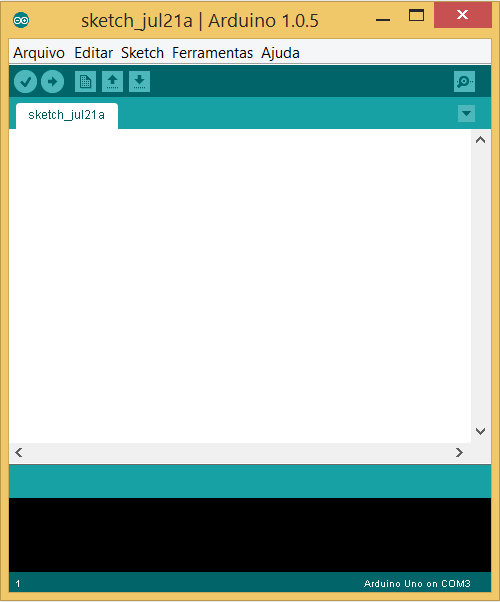
\includegraphics[width=3.7cm]{./include/chapters/sections/soft/section3/img/ide.png}
\caption{IDE Arduino}
\end{figure}
%Fim Figura
\item No Menu Sketch, selecione a opção Add Library;
%Figura
\begin{figure}[!htbp]
\centering
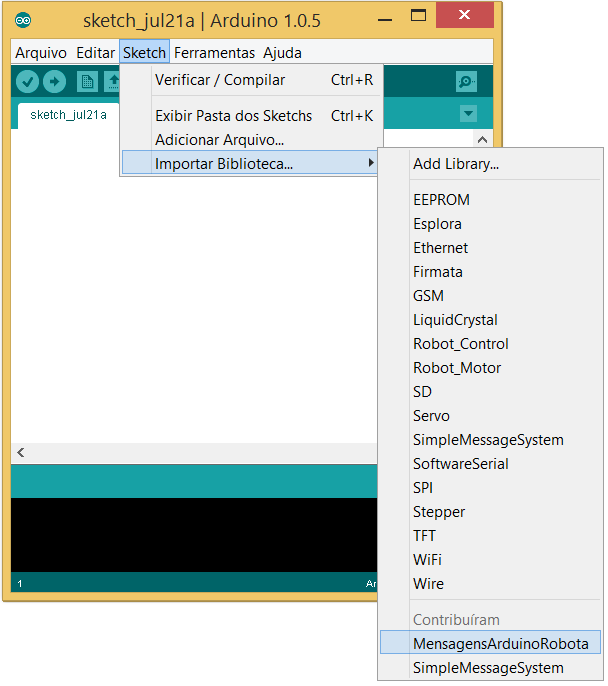
\includegraphics[width=4.5cm]{./include/chapters/sections/soft/section3/img/libadd.png}
\caption{Adicionar Biblioteca}
\end{figure}
%Fim Figura
\item Pronto. A biblioteca está adicionada. Agora é possível inclui-la no projeto com um simples include, como por exemplo 
\begin{lstlisting}
#include <MensagensArduinoRobota.h>
\end{lstlisting}
%Figura
\begin{figure}[!htbp]
\centering
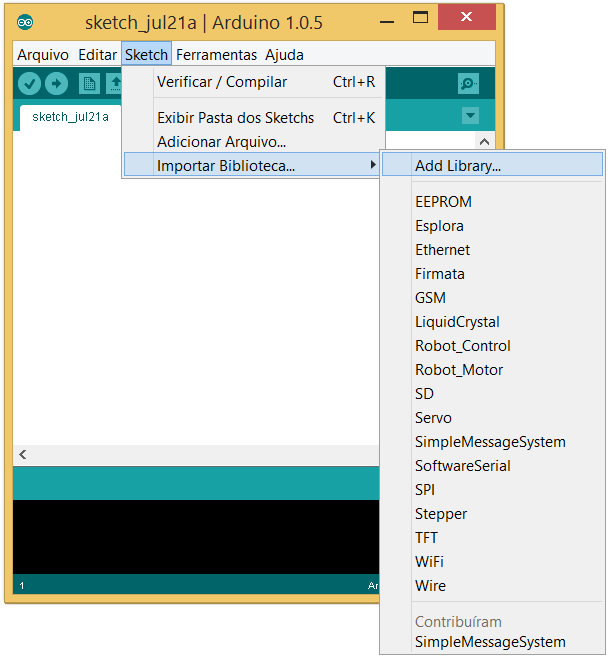
\includegraphics[width=4.5cm]{./include/chapters/sections/soft/section3/img/addlib.png}
\caption{Biblioteca adicionada}
\end{figure}
\end{enumerate}

Outra opção, um tanto menos sutil, é adicionar a pasta da biblioteca na pasta libraries no diretório onde o Arduino está instalado.

\subsection{Biblioteca MensagensArduinoRobota}

A Biblioteca "MensagensArduinoRobota" oferece aos usuários uma simples e intuitiva maneira de controlar um Arduino pelo computador.

\subsubsection{Funcionalidades}

As seguintes funcionalidades estão disponíveis:
\begin{itemize}
\item[•] Ler pinos digitais do Arduino;
\item[•] Ler pinos analógicos do Arduino;
\item[•] Chavear pinos digitais do Arduino;
\item[•] Escrever valores nos pinos de PWM do Arduino;
\end{itemize}

\subsubsection{Comandos}

Os comandos funcionam da seguinte forma:

O Arduino recebe uma string, pega a primeira letra de cada palavra para identificar o comando desejado e executa os comandos.

Os comandos resumem-se a:
\begin{itemize}
\item r $\to$ leitura
\item w $\to$ escrita
\item a $\to$ analógico
\item d $\to$ digital
\item t $\to$ todos
\item p $\to$ pino especifico para leitura
\end{itemize}

\subsubsection{Exemplos de comandos aceitos}

Alguns exemplos de comandos aceitos pela biblioteca:

\begin{itemize} 
\item r a t $\to$ Le todos os pinos Analogicos
\item r a p [pin] $\to$ Le valor do pino analogico especificado
\item r d t $\to$ Le todos os pinos digitais
\item r d p [pin] $\to$ Le valor do pino digital especificado
\item w d [pin] [value] $\to$ write digital pin
\item w a [pin] [value] $\to$ write analog pin
\end{itemize}

\subsubsection{Bibliografia}

Para a criação da presente biblioteca, os seguintes protocolos foram utilizados como exemplo:

\begin{itemize}
\item  Protocolo Firmata
\item  Protocolo CmdMessenger
\item  Protocolo SimpleMessagingSystem
\end{itemize}

\subsection{Visual C++ e Portas Seriais}

A utilização do Visual C++ para usos com o Arduino não é a maneira mais convencional encontrada, mas é uma possibilidade para alguns usuários. Existem diversas implicações negativas na escolha dessa linguagem de programação, mas existem alguns pontos positivos também. Apesar de não se ter a liberdade e praticidade que se tem ao trabalhar com periféricos via USB em S.O.s como o Ubuntu, o Visual C++ é uma alternativa funcional para utilizar C++, periféricos USB e o sistema Windows.

\subsubsection{Exemplo Visual C++ $\Rightarrow$ Porta Serial}

A seguir, exemplos simples do C++ no Windows para o controle de um Arduino conectado em uma porta USB de um PC.

O primeiro passo é adicionar uma biblioteca bastante importante para o uso de C++ e o Windows.
\begin{lstlisting}
// Biblioteca da malvada Microsoft para fazer tudo funcionar
#include "stdafx.h"
\end{lstlisting}

Com a biblioteca adicionada, é interessante definir os namespaces utilizados.
\begin{lstlisting}
using namespace System;
using namespace System::IO::Ports;
\end{lstlisting}

Agora, é possível definir a porta utilizada. No caso, a porta serial será chamada de Arduino para facilitar o processo.

\begin{lstlisting}
// Configuracao do Arduino
	int baudRate = 9600;
	portName = "COM3";
	SerialPort^ arduino;
	arduino = gcnew SerialPort(portName, baudRate)
\end{lstlisting}

É importante definir limites de tempo para a leitura e escrita de dados do Arduino.

\begin{lstlisting}
	arduino->ReadTimeout = 1500;
	arduino->WriteTimeout = 1500;
\end{lstlisting}

Para escrever algo na porta serial.

\begin{lstlisting}
	arduino->WriteLine("Algo");
\end{lstlisting}

Para ler algo da porta serial.

\begin{lstlisting}
	arduino->ReadLine();
\end{lstlisting}
\section{Documentação Doxygen e o Doxywizard}

O Doxygen é um gerador de documentação, ou seja, uma ferramenta utilizada para a redação de documentos acerca de um software. O conteúdo da documentação é escrito no corpo do código, o que facilita o referenciamento de partes do código no documento.

\subsection{Uso}

Além de aceitar a sintaxe do Javadoc, o Doxygen suporta marcações de documentação usadas no Qt toolkit e a sua saída pode ser em HTML, CHM, RTF, PDF, LaTeX, PostScript ou man pages (páginas de manual).

\subsection{Doxywizard}

Doxywizard é uma interface para a configuração e o uso do Doxygen.
Ao ser inicializado, o Doxywizard mostrará sua janela principal. Algumas diferenças visuais poderão ser notadas nos diferentes Sistemas Operacionais utilizados (caso suportados). 
\begin{figure}[!htb]
\centering
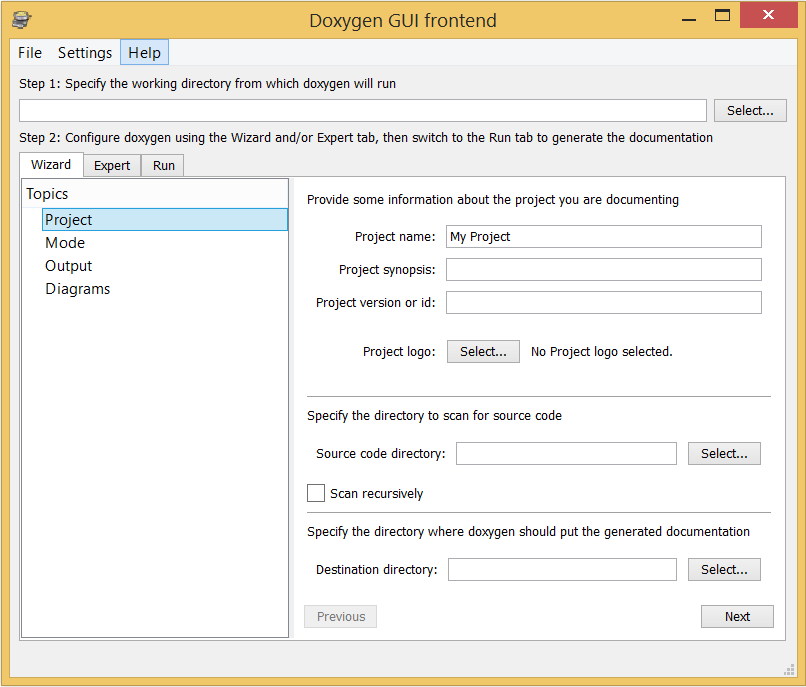
\includegraphics[width=7cm]{./include/chapters/sections/soft/section4/img/janela.png}
\caption{Janela Principal}
\end{figure}\\
Esta janela mostra os passos para realizar a configuração e a utilização do Doxygen. O primeiro passo é escolher uma das opções de configuração:
\begin{itemize}
\item  Wizard: Utilizado para configurar rapidamente as opções mais importantes e manter o restante das opções em seus padrões;
\item  Expert: Utilizado para ter acesso a todas as opções configurações;
\item  Run: Utilizado para gerar a documentação após realizadas as configurações.
\end{itemize}
É possível (e comum) realizar uma configuração básica utilizando o Wizard e realizar ajustes específicos no modo Expert.
\subsubsection{Wizard}
A aba Wizard comummente está selecionada ao iniciar-se o Doxygen, podendo ser vista na Figura 2.9. 
\subsubsection{Project}
Quando selecionada, a aba Wizard permite acesso às seguintes opções:
\begin{itemize}
\item  Determinar informações como nome, uma pequena sinopse, versão do código e logotipo do projeto;
\item  Especificar o diretório do código;
\item  Especificar o diretório alvo do documento gerado.
\end{itemize}
\subsubsection{Modes}
\begin{figure}[!htb]
\centering
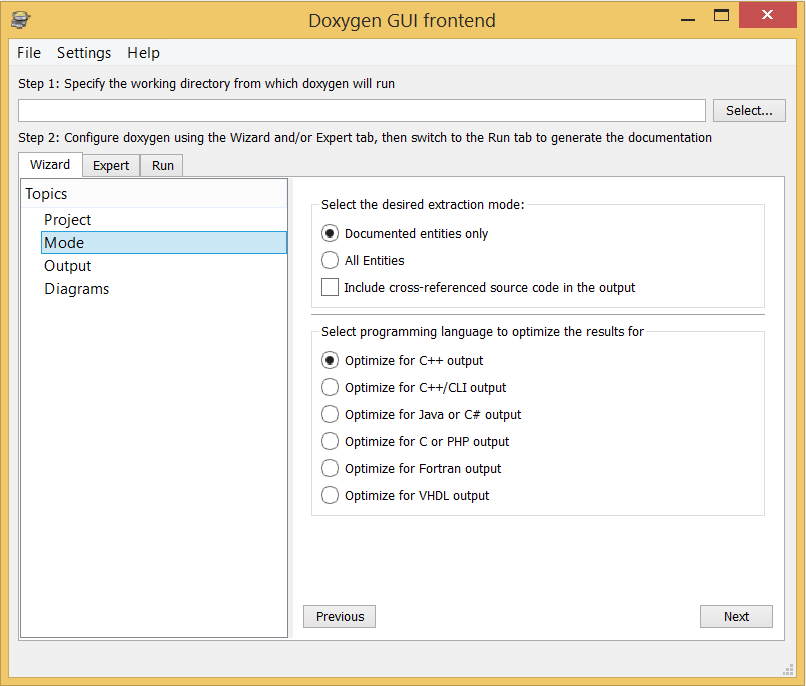
\includegraphics[width=6.5cm]{./include/chapters/sections/soft/section4/img/mode.png}
\caption{Modes}
\end{figure}
No tópico Modes é possível configurar algumas opções referentes à linguagem de programação utilizada.
\subsubsection{Output}
Tópico onde são realizadas configurações (como formato, cores e tipos) do documento gerado.
\begin{figure}[!htb]
\centering
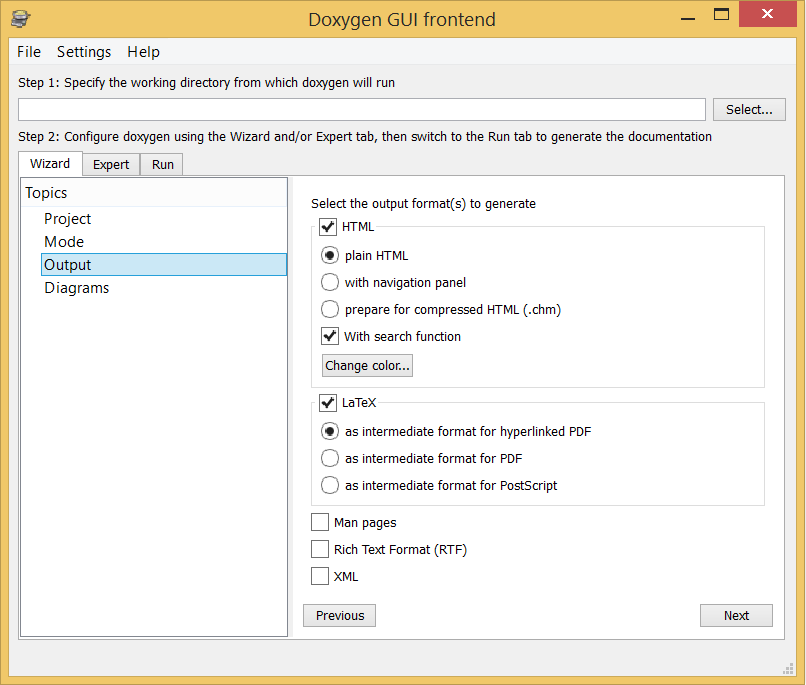
\includegraphics[width=6.5cm]{./include/chapters/sections/soft/section4/img/output.png}
\caption{Outputs}
\end{figure}
\subsubsection{Diagrams}
Tópico relacionado à diagramas.
\begin{figure}[!htb]
\centering
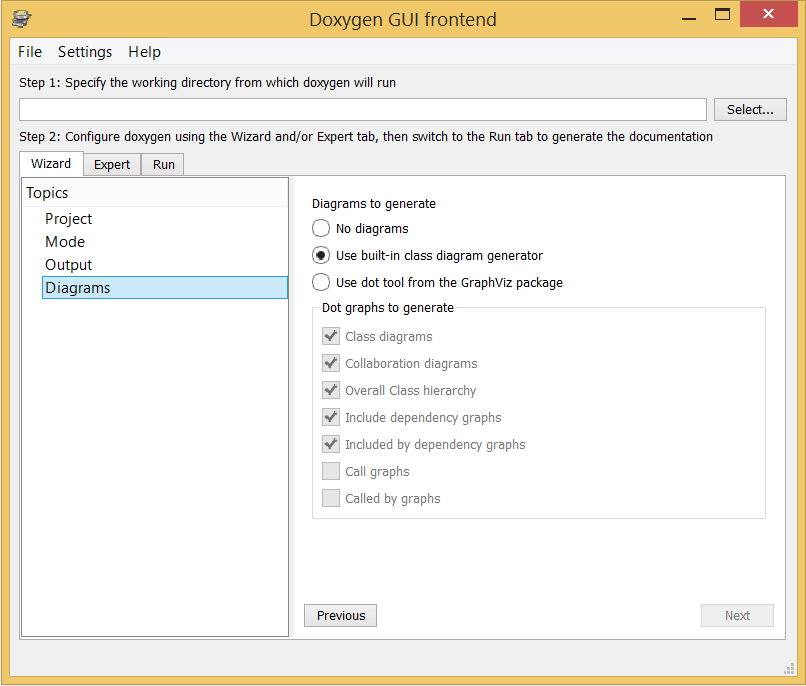
\includegraphics[width=7.2cm]{./include/chapters/sections/soft/section4/img/diagrams.png}
\caption{Diagramas}
\end{figure}

\subsubsection{Expert}

A aba Expert oferece opções de configuração mais detalhadas e avançadas.
\begin{figure}[!htb]
\centering
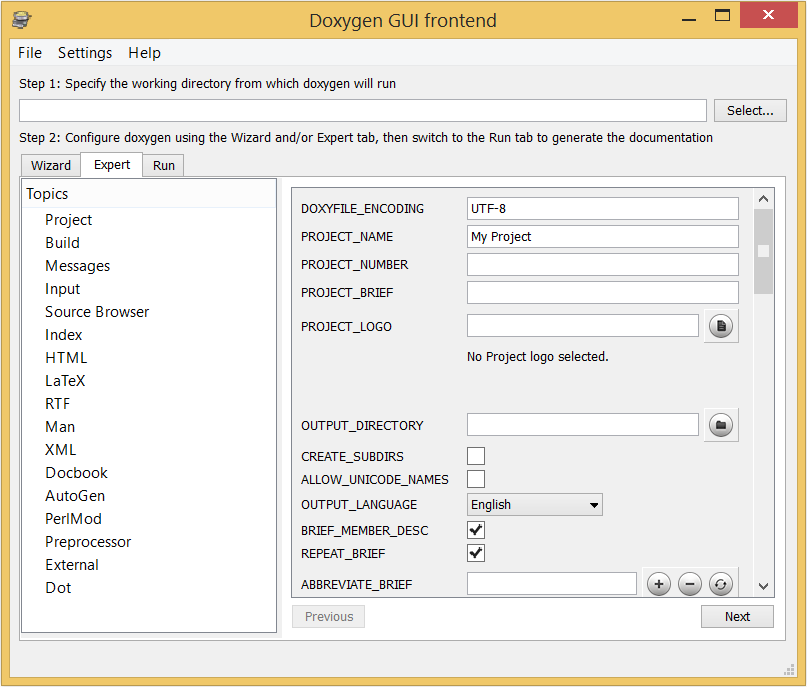
\includegraphics[width=7.2cm]{./include/chapters/sections/soft/section4/img/expert.png}
\caption{Expert}
\end{figure}

\subsubsection{Run}

A aba Run permite a geração da documentação.
\begin{figure}[!htb]
\centering
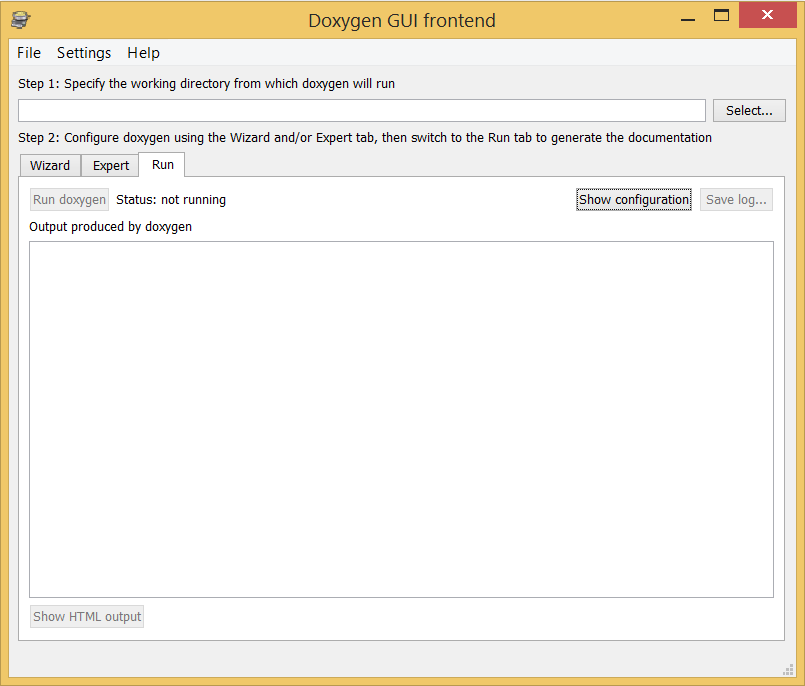
\includegraphics[width=7.2cm]{./include/chapters/sections/soft/section4/img/run.png}
\caption{Run}
\end{figure}

%----------------------------------------------------------------------------------------
% HARDWARE
\newpage
\chapter{Hardware}

Aqui seria a parte de Hardware

\section{B\'asico}

Aqui ser\~ao apresentados alguns dos conceitos b\'asicos necess\'arios para a compreens\~ao das principais aplicaç\~oes de eletr\^onica em rob\'otica m\'ovel.

\subsection{Elementos b\'asicos}


\begin{enumerate}
\item Resistor:
	O elemento mais utilizado na confecç\~ao de circuitos eletr\^onicos, é um componente chave pois permite limitar a corrente el\'etrica que passa por elementos em s\'erie, e possibilita a aplicaç\~ao de uma tens\~ao desejada atrav\'es do conceito de divisor de tens\~ao.
		\\Por definiç\~ao \'e um componente que oferece uma oposiç\~ao \`a passagem de corrente el\'etrica, dissipando energia atrav\'es do efeito Joule.
		
\item Capacitor: 
	O capacitor \'e um elemento que armazena energia na forma de campo el\'etrico, criando uma diferença de potencial entre os seus terminais. Apesar de aparentemente possuir aplicaç\~ao apenas em circuitos em corrente alternada, \'e de extrema import\^ancia nos circuitos de corrente cont\'inua. Sua aplicaç\~ao mais utilizada \'e na filtragem dos sinais, ajudando a evitar ripples e interfer\^encias indesejadas. Nesse \^ambito pode-se citar os capacitores de desacoplamento, que geralmente ficam em paralelo com a alimentaç\~ao dos chips eletr\^onicos, e evitam variaç\~oes de tens\~ao ou interfer\^encias sobre o mesmo. Um valor t\'ipico de capacitor de desacoplamento \'e de 100nF.
	
\item Diodo:
	O diodo \'e um elemento composto de cristal semicondutor, tipicamente de germ\^anio ou sil\'icio, sendo o mais simples dos elementos semicondutores, por ser composto apenas por um cristal N e um cristal P. Suas aplicaç\~oes mais importantes est\~ao relacionadas com sua caracter\'istica de conduzir apenas quando for polarizado de forma direta, ou seja, a corrente passa apenas em um sentido pelo diodo (o que explica a sua simbologia, uma seta, que aponta para o sentido da corrente passante). Outra caracter\'istica importante \'e a queda de tens\~ao que ocorre entre os seus terminais, que \'e tipicamente de 0,7V (no cristal de sil\'icio, o mais utilizado), e que varia dependendo do material semicondutor empregado.
	\\Uma aplicação cl\'assica \'e a ponte de diodos, que permite que uma tens\~ao alternada passe a ter apenas tens\~oes positivas (faz um rebatimento dos semi-ciclos negativos no eixo x). Esse sinal pode ser então regulado e filtrado (utilizando reguladores da fam\'ilia 78XX e capacitores, por exemplo). Esse \'e o princ\'ipio de funcionamento de fontes lineares (que convertem a tens\~ao da rede em tens\~ao cont\'inua).
	
\item Transistor:
	O transistor \'e um componente eletr\^onico que revolucionou a eletr\^onica por volta dos anos 60, por apresentar uma alternativa mais compacta \`as v\'alvulas e rel\'es, al\'em de possuir uma autonomia muito maior por ter seu funcionamento baseado nos efeitos de campo do seu material semi-condutor. Pode ser utilizado como chave (deve estar trabalhando na zona de saturaç\~ao) ou como amplificador (deve estar trabalhando na zona linear).
\end{enumerate}

\subsection{Aplicaç\~oes em Rob\'otica M\'ovel}

A eletr\^onica se mostra de extrema import\^ancia no \^ambito da rob\'otica m\'ovel, estando presente em praticamente todos os m\'odulos que juntos comp\~oe um rob\^o.
Logo abaixo est\~ao listados alguns exemplos de aplicaç\~ao de elementos e circuitos eletr\^onicos em um rob\^o.
\\Primeiramente haver\'a uma abordagem sobre sensores e atuadores, que basicamente s\~ao elementos que possibilitam todo tipo de interaç\~ao do rob\^o com o ambiente, cada vez mais necess\'aria \`a medidada em que a ``intelig\^encia" dos rob\^os aumenta. Logo ap\'os ser\~ao abordados os microcontroladores e computadores que s\~ao cada vez mais embarcados nos rob\^os (e em tudo o que se possa pensar no mundo), e s\~ao como um c\'erebro do rob\^o (talvez n\~ao seja o termo mais adequado, j\'a que com a diminuiç\~ao nos preços de microcontroladores o processamento de dados est\'a sendo mais distribuido em processadores pr\'oximos aos diversos elementos do rob\^o).

\begin{enumerate}
\item Sensores:
	Sensores s\~ao dispositivos sens\'iveis \`a fen\^omenos f\'isicos ou qu\'imicos, transformando-os em uma grandeza mensur\'avel. Nos seres vivos notamos a existência de diversos sensores, permitindo a interaç\~ao do organismo com o meio exterior (a vis\~ao, por exemplo utiliza sensores para interpretar as cores atrav\'es da frequ\^encia dos f\'otons de luz, os cones, e outros sensores para a luminosidade atrav\'es da quantidade de f\'otons de luz, os bastonetes).
	Quando o sensor converte esse fen\^omeno em um sinal el\'etrico (de tens\~ao ou corrente), ele \'e chamado de transdutor. Em suma, todos os sensores utilizados em rob\'otica m\'ovel s\~ao transdutores, logo necessitam de um circuito eletr\^onico para interpretar a grandeza medida, podendo ser apenas um comparador anal\'ogico utilizando amplificadores operacinais ou um circuito microcontrolado para tratar o sinal de sa\'ida do sensor. Atualmente a segunda opç\~ao, microcontrolada \'e amplamente utilizada, devido \`a reduç\~ao dos preços dos microcontroladores, e \`as vantagens relacionadas, como a transmiss\~ao de dados de forma digital (sinais alan\'ogicos s\~ao mais sucet\'iveis a ru\'idos e interfer\^encias).
	Uma tend\^encia j\'a amplamente aplicada \'e a de sensores inteligentes, que s\~ao sensores com um microcontrolador embarcado, agregando funcionalidades interessantes, como a digitalizaç\~ao dos dados, e possibilitando outras, nem sempre utilizadas, como a calibraç\~ao do sensor, supervis\~ao de valores limite, compactaç\~ao de dados e eliminaç\~ao de redund\^ancias, filtragem digital do sinal, correç\~ao autom\'atica de erros sistem\'aticos (não linearidade, dependências de temperatura, etc).\cite{apostilaStemmer}
	
\item Atuadores:
	\begin{quote}
	Atuador é um elemento que produz movimento, atendendo a comandos que podem ser manuais, elétricos ou mecânicos. Como exemplo, pode-se citar atuadores de movimento induzido por cilindros pneumáticos (pneumática) ou cilindros hidráulicos (Hidráulica) e motores (dispositivos rotativos com acionamento de diversas naturezas).
	\\- http://pt.wikipedia.org/wiki/Atuador
	\end{quote}
	Dentre estes atuadores citados, os que envolvem diretamente conceitos e circuitos eletr\^onicos s\~ao os motores, do tipo el\'etrico, sendo tamb\'em os mais utilizados no \^ambito da rob\'otica m\'ovel.
	
\item Microcontroladores:
	Um microcontrolador \'e um pequeno computador com diversos perif\'ericos dentro de um \'unico chip. Enquanto um microprocessador (como os que encontramos dentro dos PC's) apresenta apenas a ULA (unidade de l\'ogica aritm\'etica) e registradores, o microcontrolador apresenta mem\'orias EEPROM e RAM, conversores anal\'ogico-digital, interfaces de entrada-sa\'ida, clock interno e outros elementos. Obviamente por apresentar v\'arios elementos dentro do mesmo chip, eles n\~ao s\~ao t\~ao eficientes quanto um microprocessador, e trabalham em frequ\^encia muito mais baixa, na ordem de MHz, por\'em s\~ao extremamente pr\'aticos por n\~ao necessitarem de perif\'ericos externos para funcionar, serem de baixo custo e permitirem a gravaç\~ao dos programas diretamente no chip.
	\\Existem microcontroladores com diversas capacidades de processamento, o que tamb\'em influencia seu preço. Primeiramente temos os processadores de 8 bits, utilizados em aplicaç\~oes que n\~ao exigem muito poder de processamento, como o tratamento de um sinal anal\'ogico (de um sensor, por exemplo) ou o controle de um motor. Nessa categoria os microcontroladores mais populares s\~ao os PICs da fam\'ilia 16F e 18F, que s\~ao microcontroladores de arquitetura RISC (reduced instruction set computing), que funcionam em frequências de cerca de 4MHz a 20Mhz e possuem diversos perif\'ericos como conversores AD, protocolos de comunicaç\~ao implementados em hardware (USART, I2C, SPI e no caso de alguns 18Fs, USB), PWM (pulse width modulation), etc.
	
\item Computadores:


\end{enumerate}



\section{Placa de Circuito Impresso}
Nesa seç\~ao ser\'a abordado um tema de extrema import\^ancia para a eletr\^onica, que \'e relativo \`as placas de circuito impresso, que a partir de agora ser\~ao chamadas de PCB, do ingl\^es 'printed circuit board'. Saber confeccionar uma PCB significa transformar um circuito desenhado no papel em realidade, e envolve uma vasta gama de conhecimento, que ser\'a (\`a medida do poss\'ivel) condensado e resumido aqui.

\subsection{O que \'e?}

A PCB \'e uma placa, geralmente de fenolite, podendo ser tamb\'em de fibra de vidro ou de poli\'ester, com uma fina camada de cobre que \'e corro\'ida de forma a criar caminhos para conectar eletricamente componentes eletr\^onicos (chamados de trilhas), formando assim o circuito eletr\^onico desejado. A PCB foi criada para substituir a ponte de terminais, que era utilizada anteriormente, e que impedia a implementaç\~ao de circuitos mais complexos, devido aos diversos problemas de interfer\^encia e pela pr\'opria disposiç\~ao f\'isica dos componentes, que muitas vezes beiravam o caos. Outro problema encontrado nessa t\'ecnica arcaica era a produç\~ao em s\'erie dos circuitos, um processo dif\'icil de ser mecanizado e bastante meticuloso.
\\Inicialmente o desenho do circuito na placa (layout) era feito manualmente, com o aux\'ilio de r\'eguas que continham os moldes dos principais componentes utilizados, e as trilhas eram desenhadas \`a m\~ao com uma caneta permanente ou com o aux\'ilio de fitas adesivas. Obviamente hoje em dia existem softwares de computador, chamados CADs (computer aidded design) que possibilitam esse projeto. Ap\'os possuir o  layout pronto, pode-se mandar produzir as placas em alguma empresa especializada, que utiliza ferramentas avançadas possibilitando placas complexas e com componentes pequenos, ou pode-se utilizar m\'etodos artesanais para produzir essa placa, que acaba limitando a complexidade do projeto, por\'em \'e suficiente para v\'arias aplicaç\~oes interessantes.

\subsection{Elementos b\'asicos}

Aqui ser\~ao apresentados alguns conceitos e termos utilizados de forma a possibilitar o entendimento dos t\'opicos subsequentes.

\begin{enumerate}

\item Trilha: As trilhas s\~ao `caminhos' de cobre que fazem as ligaç\~oes el\'etricas necess\'arias nas placas. Sua largura est\'a relacionada com a corrente que deve passar por ela, devendo ser gradativamente mais larga ao se esperar maiores valores de corrente, e esta deve ser uma preocupaç\~ao do respons\'avel pelo layout. O risco de subdimensionar a largura da trilha \'e de, quando uma corrente muito grande passar, o cobre esquentar muito e descolar da placa, podendo at\'e mesmo fundir e romper. Isso ocorre pois a resist\^encia el\'etrica associada \'e inversamente proporcional \`a largura da trilha, e pela lei de Joule o calor dissipado \'e maior com o aumento da resist\^encia (mantendo-se a corrente passante).

\item Camadas (layers): As camadas de cobre presente em uma PCB s\~ao chamadas layers. As placas mais simples possuem apenas uma camada de cobre e s\~ao chamadas single-layer, sendo as mais utilizadas por hobbistas que utilizam processos caseiros de fabricaç\~ao das placas. Quando a placa possui duas camadas de cobre \'e chamada de dual-layer, e pode tamb\'em ser confeccionada com m\'etodos caseiros, por\'em com mais dificuldade, pois deve-se projetar o layout para os dois lados e depois sincroniz\'a-los para que os furos coincidam. Quando a placa possui mais de duas camadas \'e chamada multi-layer, e s\'o pode ser feita atrav\'es de processos industriais, com a utilizaç\~ao de materiais e m\'aquinas espec\'ificas para tal.

\item Componentes Through-Hole: S\~ao componentes que se utilizam de pinos met\'alicos que devem atravessar a placa atrav\'es de um furo, podendo ser metalizado ou n\~ao, sendo soldados no lado oposto ao componente.

\item Componentes SMD: Os componentes SMD (surface mount devices, ou dispositivos de montagem superficial), s\~ao componentes que s\~ao soldados diretamente sobre a face de cobre da PCB, sem utilizar furos para sua fixaç\~ao mec\^anica.

\item Ilhas (pads): As ilhas s\~ao superf\'icies de cobre onde os componentes s\~ao soldados. Geralmente s\~ao redondas para componentes through-hole e quadradas para os SMD.



\end{enumerate}

\subsection{CADs}

Os CADs (computer aidded design) s\~ao softwares que auxiliam no projeto e desenho t\'ecnico nas mais diversas \'areas, como no projeto de construç\~oes, de peças mec\^anicas e de PCB's, substituindo a necessidade de utilizar os processos manuais para o desenho das plantas, vistas e layouts, respectivamente. Os principais softwares do mercado oferecem ferramentas que facilitam o processo, reduzindo drasticamente o tempo de projeto e de eventuais reparos em um design j\'a existente.


\section{Softwares}
Nesta seç\~ao ser\~ao apresentados os principais softwares utilizados em aplicaç\~oes para eletr\^onica. Tais softwares s\~ao extremamente \'uteis para a realizaç\~ao de um projeto, principalmente para o projeto de placas de circuito. Esses softwares s\~ao chamados CAD's (computer aided design, ou desenho assistido em computador em portugu\^es) e geralmente permitem o projeto tanto do esquem\'atico quanto do layout da placa, tamb\'em chamado PCB (printed circuit board, ou placa de circuito impresso em portugu\^es) design. Outros softwares s\~ao utilizados pra realizar a simulaç\~ao de circuitos eletr\^onicos, acabando com a necessidade de realizar certos c\'alculos manualmente, e em alguns casos agregando aspectos pr\'aticos dos elementos, como indut\^ancias, capacit\^ancias e resist\^encias que n\~ao existem nos modelos ideais. Alguns softwares agregam todas essas funcionalidades, como \'e o caso do Proteus.
Abaixo est\~ao listados alguns dos principais softwares utilizados, com uma descriç\~ao de cada um.

\subsection{Proteus}
Desenvolvido pela empresa inglesa Labcenter Electronics, o Proteus \'e provavelmente o software mais utilizado por hobistas ao redor do mundo, principalmente pela possibilidade de simulaç\~ao de diversos microcontroladores, como os PICs da microchip e Atmegas da Atmel, além de v\'arios ARMs.
O Proteus Design Suite \'e dividido em dois softwares, o ISIS e o ARES. O primeiro \'e o programa respons\'avel pelo desenho dos esquem\'aticos, al\'em das simulaç\~oes de circuitos eletr\^onicos.

\begin{figure}[htb]
\center
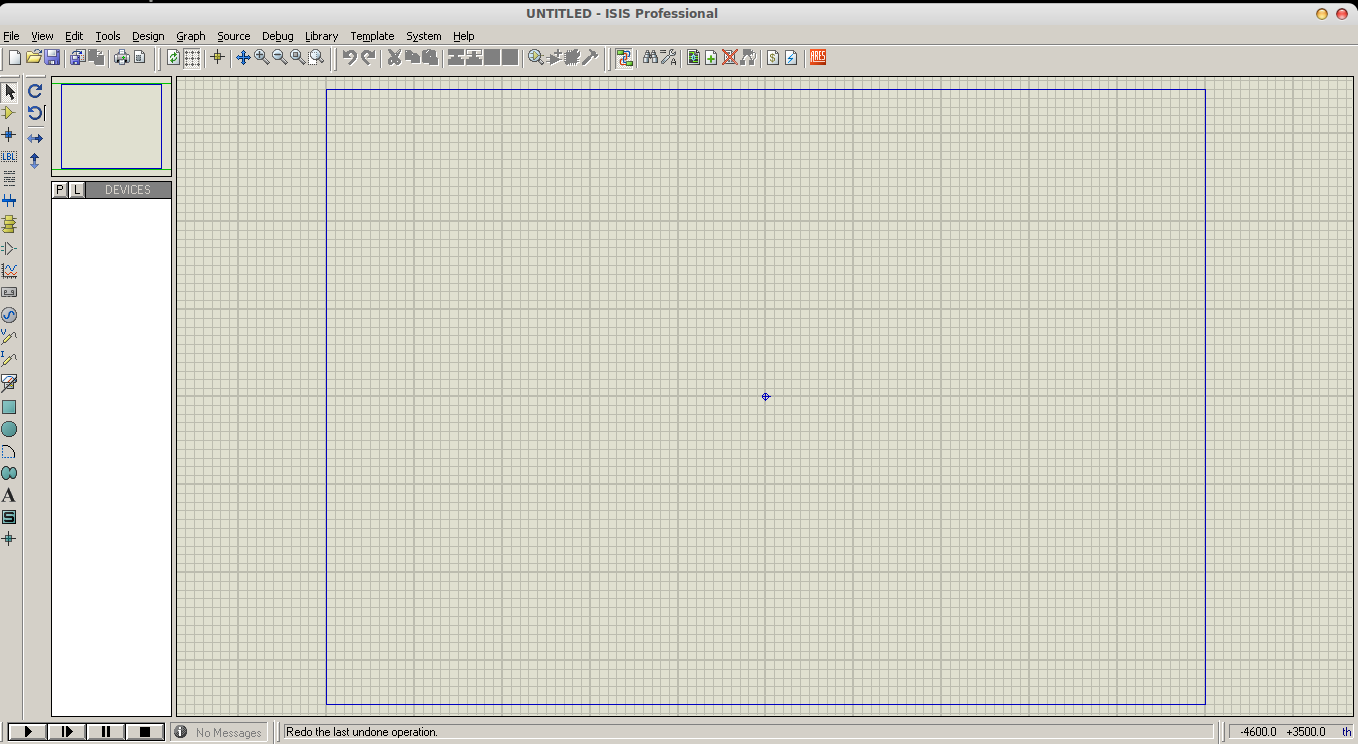
\includegraphics[width=1\textwidth]{./include/chapters/sections/hard/section1/img/Isis_homescreen.png}
\caption{Tela inicial do ISIS}
\label{IsisHome}
\end{figure}

J\'a o Ares \'e utilizado para a criaç\~ao do layout da PCB. Possui um auto-router, que roteia as trilhas automaticamente, utilizando as conex\~oes do esquem\'atico criado no ISIS. Outra funç\~ao interessante do Ares \'e a possibilidade de uma visualizaç\~ao em 3D da placa em desenvolvimento, desde que os componentes utilizados possuam um modelo em 3D.

\begin{figure}[htb]
\center
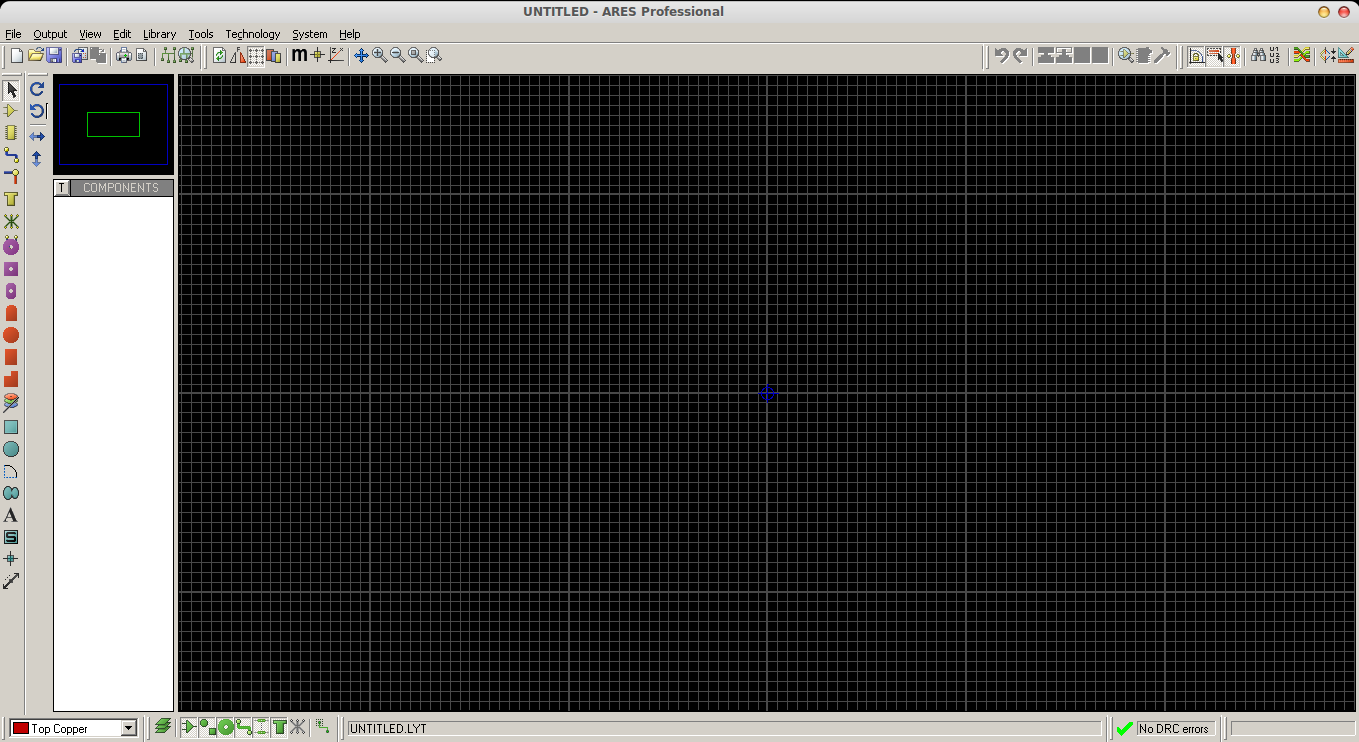
\includegraphics[width=1\textwidth]{./include/chapters/sections/hard/section1/img/Ares_homescreen.png}
\caption{Tela inicial do Ares}
\label{AresHome}
\end{figure}


\subsection{Eagle}
O Eagle (sigla de Easily Applicable Graphical Layout Editor) \'e um CAD desenvolvido pela empresa CadSoft Computer com suas primeiras ediç\~oes jur\'assicas feitas para rodar no DOS, ainda como um aplicativo de 16 bits. Atualmente possui vers\~oes para Windows, Linux e Mac OS. Possui um editor para desenhar os esquem\'aticos de cirucitos eletr\^onicos, um editor para criar o layout das placas de circuito impresso, auto-router al\'em de diversas outras ferramentas.
\\Apesar de ser um programa pago, \'e o software mais utilizado entre usu\'arios adeptos ao open source, pois sua vers\~ao freeware possui apenas uma limitaç\~ao quanto ao tamanho do projeto (que n\~ao \'e problema em aplicaç\~oes usuais), mas principalmente por possuir uma gigantesca biblioteca com os footprints dos mais variados componentes na rede, constru\'ida pelos in\'umeros hobistas que utilizam o programa.
\\\'E importante ressaltar que o Eagle \'e um programa que possui uma curva de aprendizado grande, por\'em por possuir muitos adeptos \'e f\'acil encontrar material na internet que possa ajudar a utiliz\'a-lo.

\begin{figure}[htb]
\center
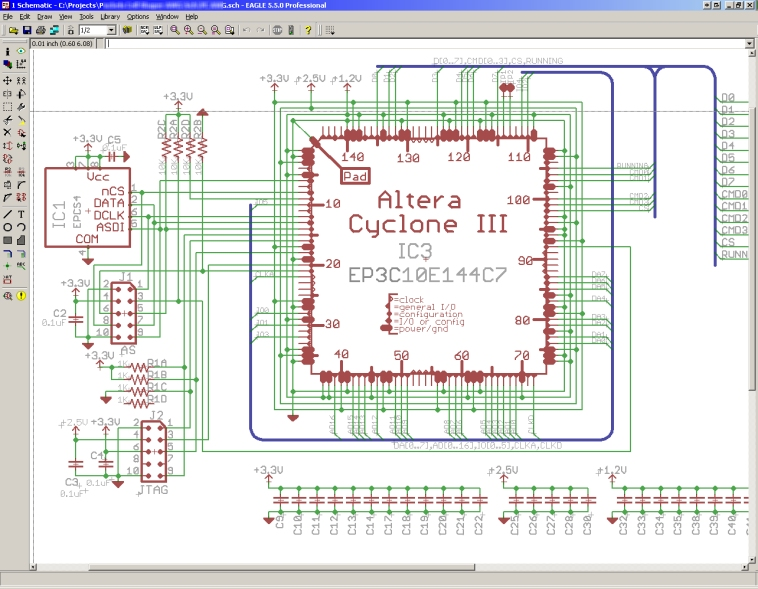
\includegraphics[width=1\textwidth]{./include/chapters/sections/hard/section1/img/Eagle_schem.jpg}
\caption{Editor de esquem\'aticos do Eagle}
\label{Eagle_schem}
\end{figure}

\begin{figure}[htb]
\center
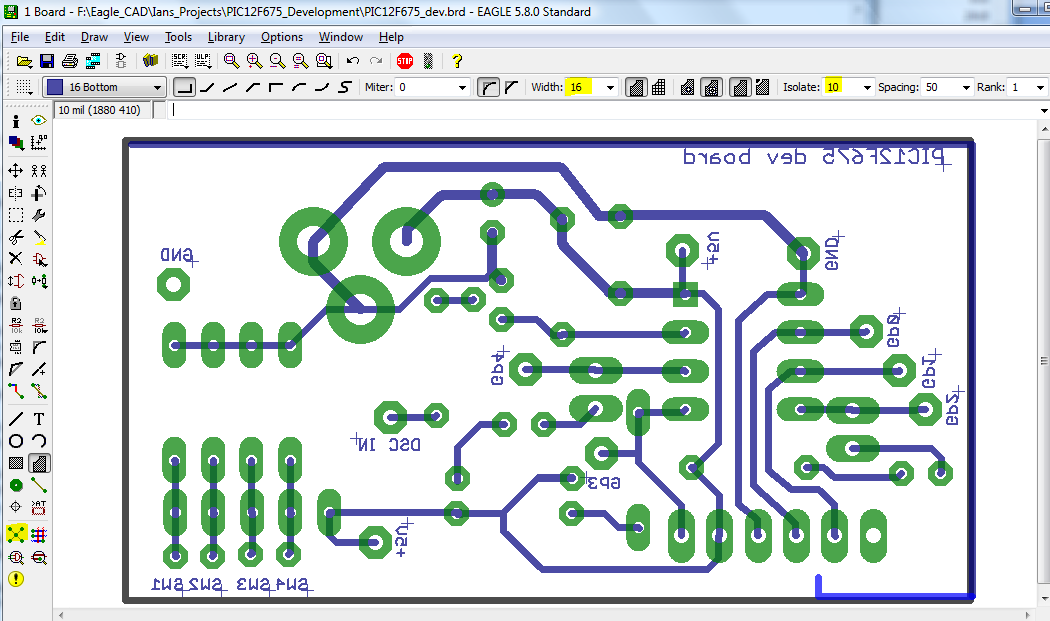
\includegraphics[width=1\textwidth]{./include/chapters/sections/hard/section1/img/Eagle_layout.png}
\caption{Editor de layout do Eagle}
\label{Eagle_layout}
\end{figure}

\subsection{Altium Designer}
Possivelmene um dos mais completos programas para desenvolvimente de projetos eletr\^onicos, sendo desenvolvido pela empresa Australiana Altium Limited, \'e baseado  no famoso Protel, um software muito utilizado at\'e o começo dos anos 2000's. Possui a mais variada mir\'iade de funcionalidades e ferramentas para o desenvolvimento de placas de circuito impresso e FPGA's. \'E recomendado para projetos complexos, lidando bem com placas com m\'ultiplas camadas e componentes SMD. Possui um poderoso visualizador 3D (na verdade foi o primeiro software a apresentar essa ferramenta, em 2007), preciso e muito \'util para averiguar corriqueiros conflitos mec\^anicos que possam ocorrer no roteamento da placa. Software utilizado por diversas empresas que produzem placas com n\'ivel de complexidade elevado, interessante para quem deseja ter contato com um software de n\'ivel profissional.

\subsection{Psim}



%----------------------------------------------------------------------------------------
% MECANICA
\newpage
\chapter{Mec\^anica}

Aqui seria a parte mec\^anica do doc

%----------------------------------------------------------------------------------------
% GERENCIA
\newpage
\chapter{Gerencial}

Aqui seria a parte de Gerenciamento

% BIBLIOGRAFIA
\bibliography{bibliography.bib}

\end{document}